% !TeX root = ../main.tex
\section{Результаты поиска сигнала}
Поиск сигнала выполнен по всей сетке $1022 \times 9$ ячеек с использованием метода быстрой циклической свертки на основе дискретного преобразования Фурье:
\begin{equation}
\mathbf{corr}(f_{\text{д}}) = \mathcal{F}^{-1}\Bigl\{ \mathcal{F}\bigl\{y_k \cdot e^{-j 2\pi (f_0 + f_{\text{д}}) k T_d}\bigr\} \cdot \mathcal{F}^*\bigl\{G(k T_d)\bigr\} \Bigr\}.
\end{equation}

Полученная двухмерная поверхность корреляционного отклика $X^2(\tau_{\text{з}}, f_{\text{д}})$ приведена на рис.~\ref{fig:search_surface}.

\begin{figure}[htbp]
\centering
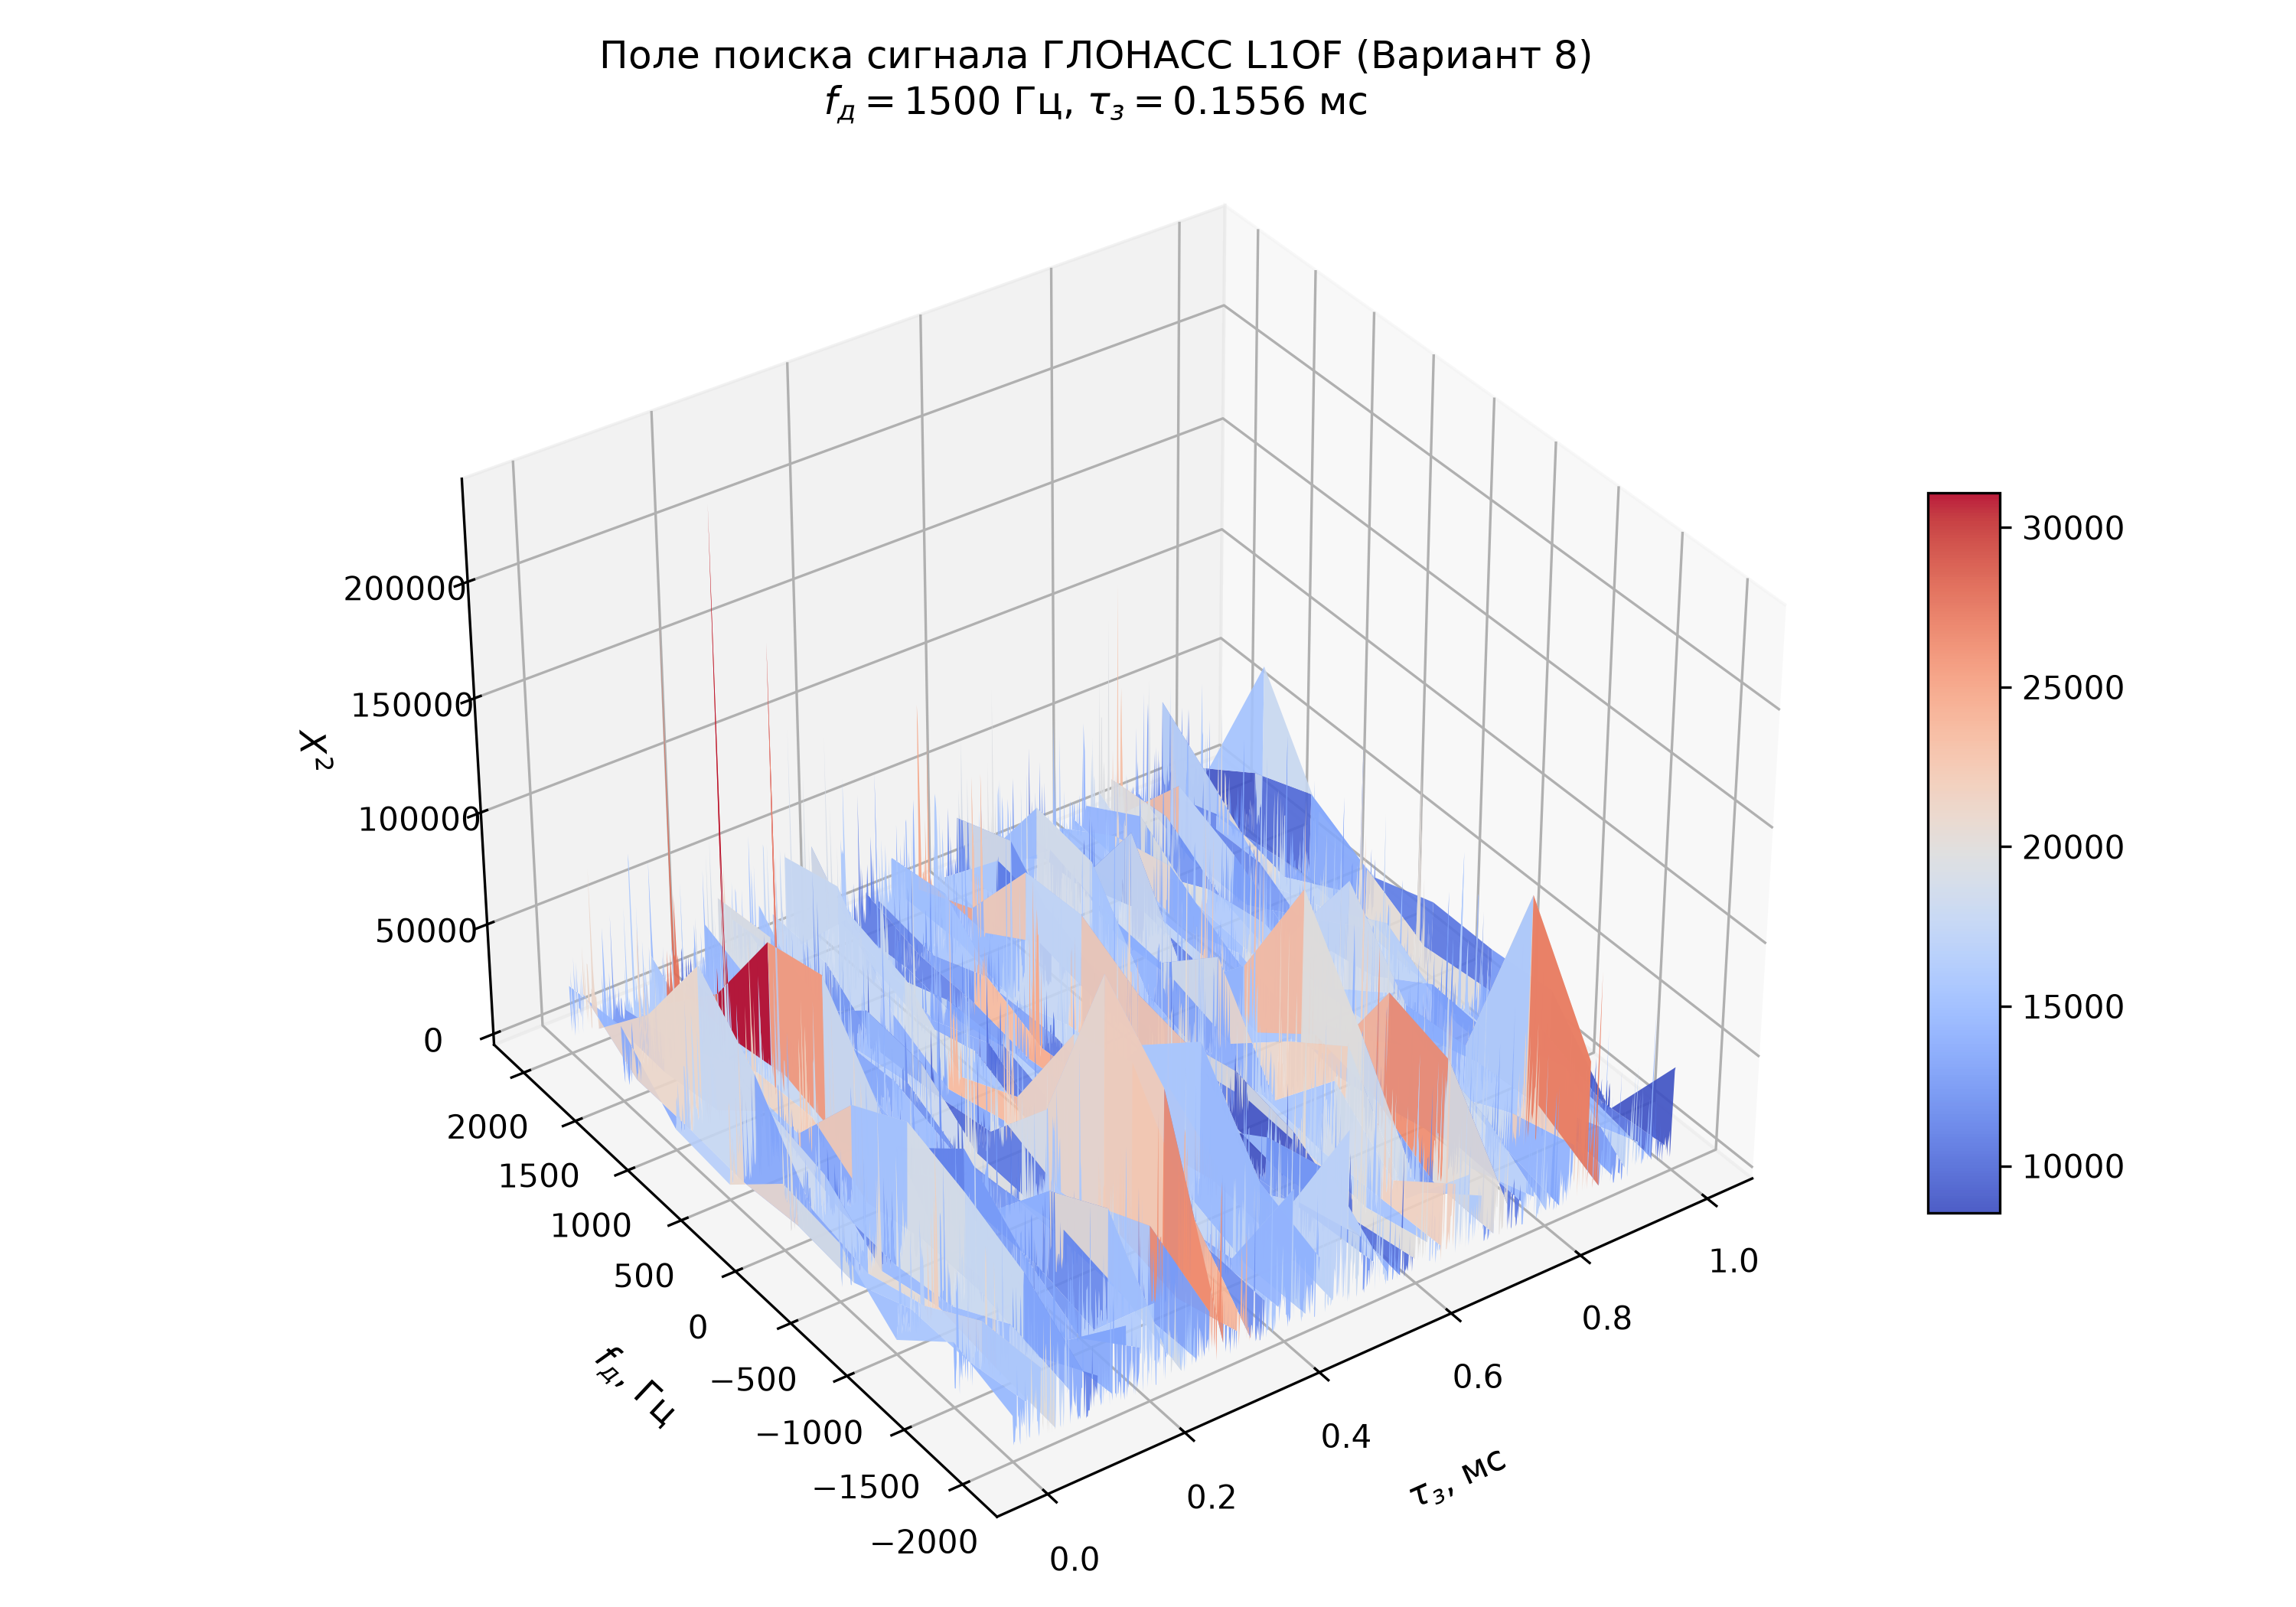
\includegraphics[width=0.85\textwidth]{search_surface_var8.png}
\caption{Поле поиска сигнала ГЛОНАСС L1OF по задержке и доплеровской частоте (Вариант 8)}
\label{fig:search_surface}
\end{figure}

По результатам анализа максимума корреляционного отклика получены следующие значения:
\begin{itemize}
    \item Максимальный корреляционный отклик: $X^2_{\max} \approx 2.45 \cdot 10^5$;
    \item Расчетный порог обнаружения ($P_{\text{ло}} = 10^{-4}$): $h \approx 1.48 \cdot 10^5$;
    \item Оценка доплеровского сдвига частоты: $\hat{f}_{\text{д}} = 1500\text{ Гц}$;
    \item Оценка времени задержки сигнала: $\hat{\tau}_{\text{з}} = 0.1556\text{ мс}$.
\end{itemize}

Условие обнаружения $X^2_{\max} > h$ уверенно выполняется. На графике четко выражен единственный глобальный корреляционный пик, превышающий фоновые шумовые флуктуации более чем в 7 раз.
